%% LyX 2.2.2 created this file.  For more info, see http://www.lyx.org/.
%% Do not edit unless you really know what you are doing.
\documentclass[english]{article}
\usepackage[T1]{fontenc}
\usepackage[latin9]{luainputenc}
\setlength{\parskip}{\smallskipamount}
\setlength{\parindent}{0pt}
\usepackage{babel}
\usepackage{graphicx}
\usepackage[unicode=true,
 bookmarks=true,bookmarksnumbered=false,bookmarksopen=false,
 breaklinks=false,pdfborder={0 0 1},backref=false,colorlinks=false]
 {hyperref}
\hypersetup{pdftitle={Power Enjoy: Design Document},
 pdfauthor={Niccolo' Raspa, Matteo Marinelli}}

\makeatletter

%%%%%%%%%%%%%%%%%%%%%%%%%%%%%% LyX specific LaTeX commands.
%% Because html converters don't know tabularnewline
\providecommand{\tabularnewline}{\\}

%%%%%%%%%%%%%%%%%%%%%%%%%%%%%% Textclass specific LaTeX commands.
\newenvironment{lyxlist}[1]
{\begin{list}{}
{\settowidth{\labelwidth}{#1}
 \setlength{\leftmargin}{\labelwidth}
 \addtolength{\leftmargin}{\labelsep}
 \renewcommand{\makelabel}[1]{##1\hfil}}}
{\end{list}}
\newcommand{\strong}[1]{\textbf{#1}}

%%%%%%%%%%%%%%%%%%%%%%%%%%%%%% User specified LaTeX commands.
\usepackage{changepage}

\makeatother

\begin{document}

\title{\emph{Power EnJoy \\
Integration Test Plan Document}\\
\vspace{12px}}

\author{Niccolo' Raspa, Matteo Marinelli}

\maketitle
\vspace*{20px}
\begin{center}
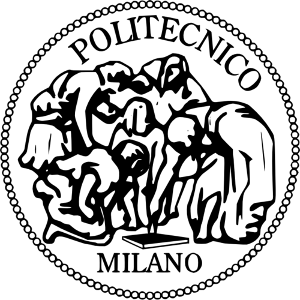
\includegraphics[scale=0.6]{../DD/images/polimi} 
\par\end{center}

\vspace{100px}
\begin{center}
Software Engineering 2 Course Project
\par\end{center}

\pagebreak{}

\tableofcontents{}

\pagebreak{}

\section{Introduction}

\subsection{Revision History}

\begin{table}[!tph]
\begin{tabular}{|c|c|c|c|}
\hline 
Version & Date & Author(s) & Summary\tabularnewline
\hline 
\hline 
1.0 & 06/01/2016 & Niccolo' Raspa, Matteo Marinelli & Initial Release\tabularnewline
\hline 
\end{tabular}

\end{table}


\subsection{Purpose and Scope}

This document represents the Integration Testing Plan Document for
PowerEnJoy. The main purpose of this document is to outline, in a
clear and comprehensive way, the main aspects concerning the organization
of the integration testing activity for all the components that make
up the system. 

This process is essential because it not only guarantees that every
component behaves as expected but also that all the components interoperate
correctly together to fullfil all the functionalities expected from
the system. 

We will focus deeply on the Application Layer since it implements
all the core of our business. This component is divided in different
services which provides great benefits but the implicit granularity
of a service oriented approach must be fully tested to guarantee that
all the subcomponents behave as one cohesive layer.

\paragraph{This document is structured as follows:}
\begin{description}
\item [{Chapter\ 1}] Provides general information about the ITPD document.
\item [{Chapter\ 2}] Explains in details the chosen integration strategy.
In more details:
\end{description}
\begin{itemize}
\item Lists of the subsystems and their subcomponents involved in this process
\item Specifies the criteria that must be met before integration testing
begins
\item Describes the integration testing approach and the rationale behind
it 
\item Outlines the order in which components and subcomponents will be integrated
\end{itemize}
\begin{description}
\item [{Chapter\ 3}] Describes the type of tests that will be used to
verify that every step of the integration process above perform as
expected.
\item [{Chapter\ 4}] Identifies all tools and test equipment needed to
accomplish the integration. 
\item [{Chapter\ 5}] Identifies any program stubs or special test data
required for each integration step
\end{description}

\subsection{List of Definitions and Abbreviations}
\begin{description}
\item [{DD:}] Design Document
\item [{RASD:}] Requirement Analysis and Specification Document
\item [{ITPD:}] Integration Test Plan Document
\item [{EJB:}] Enterprise JavaBeans
\item [{SOA:}] Service Oriented Architecture
\item [{Component:}] One of the four tier of the system (Client, Web, Application,
Database)
\item [{Subcomponent:}] Usually refers to the Application Layer, and refers
to a EJB that encapsulates a specific part of the business logic of
the module
\item [{Layer:}] synonim of \emph{Component}
\item [{Service:}] synonim of\emph{ Subcomponent}
\item [{Power\ User:}] Registered user of the application
\end{description}

\subsection{List of Reference Documents}

Please refer to the following documents, for additional informations
on the Power Enjoy System:
\begin{itemize}
\item Project rules of the Software Engineering 2 project
\item Power Enjoy - Requirement Analysis and Specification Document 
\item Power Enjoy - Design Document 
\item \strong{Documentation of any tool you plan to use for testing }
\end{itemize}
\pagebreak{}

\section{Integration Strategy}

\subsection{Entry Criteria}

This section describes the prerequisites that need to be met before
integration testing can be started.

\paragraph{Stakeholder Approval }

First of all, the Requirements Analysis and Specification Document
and the Design Document must have been presented to the stakeholders
for approval even before the coding phase can begin, this will ensure
that they're satisfied with the development.

\paragraph*{Website and Mobile App}

The presentation layer to the user might not be completed but communication
between the Application Server and Clients, both via the Mobile App
and via the Web Server, must have clearly structured and coded via
RESTful APIs using JAX-RS.

\paragraph*{Coding and Testing Application Layer}
\begin{itemize}
\item All the classes and methods of the Entity Beans must be coded and
must pass thorough \strong{Unit tests}. Unit tests should have a
minimum coverage of 90\% of the lines of code and should be run automatically
at each build using JUnit. 
\item \strong{Code inspection} has to be performed on all the code in order
to ensure maintainability, respect of conventions and find possible
issues which could increase the testers\textquoteright{} effort in
next testing phases. Code inspection should be performed using automated
tools when possible.
\item \strong{Documentation} of all classes and functions should be well
written using JavaDoc. The public interfaces of each Entity Bean shoud
be clearly stated.
\item \strong{Object relational mapping} of each service to its corresponding
database should be implemented with automated tools to avoid errors
(such as Hibernate) and fully tested.
\end{itemize}

\subsection{Elements to be Integrated}

In this section we\textquoteright re going to provide a list of all
the components that need to be integrated together. The figure below
corrispond to the system architecture already discussed in the Design
Document. 

The system is built upon the interactions of many tiers, each one
implementing a specific set of functionalities. Every tier is also
obtained by the combination of several lower-level components. This
modularity causes that the integration phase will involve the integration
of components at different levels of abstraction. In addition our
system is in relation with External Systems, which are crucial for
our application to work. It's important that they're correctly integrated
to the system in a way in which everything is trasparent to the user.

\begin{adjustwidth*}{-2cm}{-2cm}
\begin{center}
\includegraphics[scale=0.45]{images/CompletedArchitecture}
\par\end{center}

\end{adjustwidth*}

\vspace*{20px}

In summary, the elements to integrate are:
\begin{enumerate}
\item Integration of the different services inside the Application Layer.
\item Integration of different tiers (Client - Web - Application)
\item Integration and configuration with third party systems (Payment System,
Assistance System)
\end{enumerate}
\pagebreak{}

\subsection{Integration Testing Strategy}

The approach we\textquoteright re going to use to perform integration
testing is based on a mixture of the bottom-up and functional-grouping
integration strategies. This choice is due to the fact that if the
entry criteria is met, it's reasonable to assume that we have different
small services, indipendent from one other, that implement correctly
a small part of the application logic and by integrating them we're
able to create a more and more complex system that will eventually
satisfy all the requirements. In a pure bottom-up strategy we would
start from the lowest layers of the system, testing the basic functionalities,
then moving forward the most abstract layers but in our case this
approach would be unefficient. Since every service is dedicated to
one part of the business logic we can parallelize this testing, focusing
on different logic groups at the same time, giving more priority to
the critical components first and then integrating secondary functionalities.
Moreover, we also need to keep in mind that we're dealing with external
systems and if we discover some bugs or problems on their side, fixes
might take time and this would create a time gap in which we're not
able to move the integration forward.

For all these reasons we believe that the best integration strategy
is the following:

\paragraph{PHASE 1: Assure that services in relations with external systems
works as expected. \protect \\
\protect \\
}

As stated earlier, in order to avoid wasting time we start from the
boundary of the system. This process should be fairly quick if everything
was implemented as mutually agreed and should immediatly discover
issues that we can notify early on to external parties. In this phase
we'll test the communication between\emph{ Assistance Service - Assistance System}
and \emph{Payment Service - Payment System}.

\paragraph{PHASE 2: Assure that we have control over the Car \protect \\
\protect \\
}

This phase is similar to the previous, and can be carried in parallel.
In this phase we're also in relation with an external system which
is the \emph{Car On Board System} but due to the relevance of this
process we've decided to outline it and dedicated a whole phase. We
can't move the integration forward if we're lacking the foundations.
In a digital management system for a car-sharing service the control
over the car must be treated as a first class citizen. This will avoid
a big bang scenario, where we have implemented high level functionalities
that not reflect the concrete situation of the car in the real world.
These two inital phases will also allow us to ``forget'' of external
systems in the next phases, and only focus on the relation among different
services.

\pagebreak{}

\paragraph{PHASE 3: Integration of Services \protect \\
\protect \\
}

In this part the bottom-up approach would be used to build complex
functionalities integrating different services. Since subsystems are
fairly independent from one another, the order in which they\textquoteright re
integrated together to obtain the full system follows the critical-module-first
approach. This strategy allows us to concentrate our testing efforts
on the riskiest components first that represent the core functionalities
of the whole system. By proceeding this way, we are able to discover
bugs earlier in the integration progress and take the necessary measures
to correct them on time.

The most critical service to integrate is the \emph{Reservation Component}
which manages all active reservation made by Power Users, we will
ensure that it integrates correctly both with the \emph{User Component}
and the \emph{Car Service}. This will ensure that we have a stable
prototype of the actual software that implements the core functionalities.
From this prototype we will spread like wildfire, integrating other
Components that implements all the secondary functionalities.

In this phase, it is only necessary to use drivers to simulate the
top layers during the testing, which are a lot easier to produce than
stubs. 

\paragraph{PHASE 4: Integration with top layers \protect \\
\protect \\
}

In this phase we will remove the drivers and connect the Application
Side to the top tiers. We must ensure that the Application Layer works
with real inputs from the ``external word'' and not only in a simulated
and controlled environment. The integration should proceed smoothly
since the communication via RESTful APIs was clearly structured at
the beginning of the integration but we should focus deeply on errors
and expection handling.

\paragraph{PHASE 5: Alpha Test\protect \\
\protect \\
}

In this phase we'll test the Power Enjoy System as a whole. This phase
will provide a confirmation of the correctness of the integration
process and will ensure that we haven't overlooked possible error
scenarios.

\subsection{Sequence of Component/Function Integration}

NOTE: The structure of this section may vary depending on the integration
strategy you select in Section 2.3; use the structure proposed below
as a non mandatory guide

\subsubsection{Software Integration Sequence}

For each subsystem, identify the sequence in which the software components
will be integrated within the subsystem; relate this sequence to any
product features that are being built up.

\subsubsection{Subsystem Integration Sequence}

Identify the order in which subsystems will be integrated; if you
have a single subsystem, 2.4.1 and 2.4.2 are to be merged in a single
section. You can refer to Section 2.2 of the test plan example {[}1{]}
as an example

\section{Individual Steps and Test Description}

For each step of the integration process above, describe the type
of tests that will be used to verify that the elements integrated
in this step perform as expected. Describe in general the expected
results of the test set. You may refer to Chapter 3 and Chapter 4
of the test plan example {[}1{]} as an example of what we expect.
(NOTE: This is not a detailed description of test protocols. Think
of this as the test design phase. Specific protocols will be written
to fulfill the goals of the tests in this section.

\section{Tools and Test Equipment Required}

\strong{Identify all tools and test equipment needed to accomplish the integration.
Refer to the tools presented during the lectures. Explain why and
how you are going to use them. Note that you may also use manual testing
for some part. Consider manual testing as one of the possible tools
you have available.}
\begin{description}
\item [{JUnit}] Before integration testing, tests on single components
is necessary. This first part of testing is not covered in this document.
Anyway, the main issue is to check the absence of bugs and problem
in each part of the system, from the application to the all the Application
Server components. JUnit is the most used framework for single components
testing in java. In particular, we are going to use it in order to
verify that the correct objects are returned after a method invocation,
that appropriate exceptions are raised when invalid parameters are
passed to a method and other issues that may arise when components
interact with each other.
\item [{Mockito}] Mockito is an open-source test framework useful to generate
mock objects, stubs and drivers. Since the entire system interacts
with external and real objects, is necessary to use a framework to
reproduce this kind of entities. In unit testing, mock objects can
simulate the behavior of complex, real objects: they are useful when
a real object is impractical or impossible to incorporate into a unit
test. They are also useful for the developers, who have to focus their
tests on the behavior of the system without worrying about its dependencies
and having predictable results.
\item [{Arquillian}] Arquillian is an integration testing framework for
business objects that are executed inside a container or that interact
with the container as a client. We choose it as framework because
is widely used and is quite simple to work on. It combines a unit
testing framework (JUnit), and one or more sup- ported target containers
(Java EE container, etc) to provide a simple, flexible and pluggable
integration testing environment. Arquillian makes integration testing
no more difficult than the bins testing. Specifically, we are going
to use Arquillian to verify that the right components are injected
when dependency injection is specified, that the connections with
the database are properly managed and similar containerlevel tests.
\item [{Devices}] The application run on two types of operative systems
(Android and IOs). This fact make necessary testing on the direct
tools that allow users to exploit power enjoy system. Power Enjoy
service was tested on two groups of mobile devices (non necessarly
phones), one for each type of operative system. Web page is available
on the web and a group of computers were used to test the page. Test
were made on every combination of Operative system and browser.
\end{description}

\section{Program Stubs and Test Data Required}

Based on the testing strategy and test design, identify any program
stubs or special test data required for each integration step.

\section{Effort Spent}

The approximate number of hours of work for each member of the group
is the following: 
\begin{lyxlist}{00.00.0000}
\item [{Niccolo\textquoteright \ Raspa}] 5 Hours
\item [{Matteo\ Marinelli}] y Hours
\end{lyxlist}

\end{document}
